\documentclass{article}

\usepackage{parskip}
\usepackage{hyperref}
\usepackage{amsmath}
\usepackage{graphicx}
% \usepackage{caption}
\usepackage{tikz}
\hypersetup{
    colorlinks=true,
    linkcolor=blue,
    filecolor=magenta,      
    urlcolor=blue,
}

\title{MATH-2934 Project}
\author{Aaron Pierce}
\date{\today}

\begin{document}
    \maketitle

    My project takes place in two parts, each with the purpose of practicing and applying the material from Calculus III.
    I will present herein two different animations that I have programmed, demonstrating and applying examples of parametric equations, vector fields, divergence, and curl,
    as well as exploring how partial derivatives can be calculated by a computer and how Green's theorem can be understood.

    \section{Parametric Equations and Lissajous Curves}
    \underline{\href{https://saxten2011.github.io/AlmostLissajousCurves/}{View the animation here}} (should this link not work I will provide the URLs as a comment with my submission)

    This animation draws a table of Lissajous curves, a family of parametric curves that describe complex harmonic motion.
    The parameterizations of the curves are as follows:
    \begin{gather*}
        \vec{r}(t) = \left( \sin(\frac{1}{a} t),\, \cos(\frac{1}{b} t) \right)
    \end{gather*}
    Where $a$ and $b$ increase along the rows and columns of the tables, so the top left corner has minimal $a$ and $b$, and the bottom right corner has maximal $a$ and $b$.
    As well, $a$ and $b$ increase by a constant and equal amount as you move along a row or column, thus the diagonal of the table results in a parameterization of 
    $\vec{r}(t) = \left( \sin(\frac{1}{a} t), \cos(\frac{1}{a} t) \right)$, which will generate a circle, as the periods of the sine and cosine functions will be the same.

    Because $a$ and $b$ increase along the table, you can see that as you get closer to the bottom right corner of the table that the animation is slower.
    This is to be expected, as dividing the variable passed to the trigonometric functions will extend their period, and as a result making a full loop of the curve will take longer than a curve higher up on the table.

    This animation provides two interesting insights.
    Firstly, it is interesting to see how beginning with a base of the parameterization of a circle, and slightly perturbing it will produce such beautiful patterns.
    It is illuminating to watch the individual columns as they draw their curves, because the x position of the drawing point of each curve is constant along the column, so you can see very clearly the effects of the change in the functions period, as it goes slower the further down the column you move

    The second insight lies in understanding polar coordinates, surprisingly.
    Some polar curves, when graphed over the interval $[0, 2\pi)$ will repeat themselves, drawing the curve multiple times.
    This can be seen and understood in this table, as the 'velocity' of each curve in the animation shows very clearly that
    one curve could complete multiple cycles while another is still drawing its first.
    This gives an interesting perspective on polar coordinates, imagining them as having some velocity with which they graph,
    and acknowledging that curves with a faster 'velocity', or smaller period, should be suspicious for repeating themselves, as they will 'finish' faster than others.

    \section{Vector Fields, Divergence, Curl, and Approximating Partial Derivatives With a Computer}
    \underline{\href{https://saxten2011.github.io/VectorField/}{View the animation here}} (should this link not work I will provide the URLs as a comment with my submission)

    This animation depicts a vector field with particles moving along the 'flow' described by the arrows of the field, where bright colors of vectors mean a high magnitude of the vector at that point.
    The vector field is given by the following:
    \begin{gather*}
        \vec{ \mathbf{F} } (x, y) = (y \cos(y), \cos(xy)) 
    \end{gather*}

    This vector field has a number of interesting features that made it ideal for selection.
    Firstly, the top and the bottom of the graphed region are regions with a high velocity of flow, which contrast themselves with the slower center.
    The middle region very clearly has a point with highly positive curl, as you can see the particles swirling around it like a whirlpool.

    \begin{figure}[!h]
        \centering
        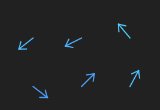
\includegraphics{whirlpoolish}
        \caption{A rough whirlpool arrangement of vectors, though a bit rotated, the idea can be seen}
    \end{figure}

    Seeing this whirlpool was the main intention of the animation, giving a strong visual intuition of what curl actually looks like.
    We can see from the vectors around the point with high curl, that a point with strong curl should look roughly like the figure above.
    All of the vectors are pointing to the next, so that a particle that travels along them will follow the whirlpool.
    The above figure is a little tilted, though, the following is a more ideal arrangement of such a whirlpool:

    \begin{figure}[!h]
        \centering
        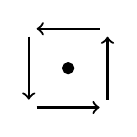
\begin{tikzpicture}
            \draw[black, thick, ->] (0, 0.9) -- (0, 0.1);
            \draw[black, thick, ->] (0.9, 1) -- (0.1, 1);
            \draw[black, thick, ->] (1, 0.1) -- (1, 0.9);
            \draw[black, thick, ->] (0.1, 0) -- (0.9, 0);
            \filldraw [black] (0.5, 0.5) circle (2pt);
        \end{tikzpicture}
        \caption{A point on the vector field shown with its neighboring vectors. We would say that the curl at the point is high because of the whirlpool arrangement of vectors around it}
    \end{figure}

    This is very close to what is seen in the animation.
    The animation's vectors are rotated a bit, so this square would look like it had been rotated about 30 degrees, but the idea holds.

    This figure gives us the ideal circumstances for curl, and from it we can derive the formula for two dimensional curl.
    Because curl will occur when vectors around a point look like the figure, describing what properties this figure has will give us an intuitive definition for curl in two dimensions.

    Firstly, we see that moving from left to right across the point moves from a negatively pointing vector to a positively pointing vector.
    These vectors point in the y direction, so we can represent this information by taking a partial derivative of the $y$ component of the vector field by $x$, which when notated looks like
    $\frac{\partial Q}{\partial x}$
    In other words, how the y component of the vector changes as you move along the $x$ direction.

    Similarly, we see that moving from the bottom to the top of the point takes a positive vector to a negative vector, thus we look for 
    $\frac{\partial P}{ \partial y}$, and hope that it is negative.
    
    To represent this information, we can subtract the two partial derivatives, 
    because we \emph{want} $\frac{\partial P}{ \partial y}$ to be negative. When we subtract this negative number, the overall result will be a higher number, and will correspond to more curl, which is exactly what we want.

    Therefore we arrive at the formula for two dimensional curl.
    \begin{gather*}
        \text{curl}_\text{2D} =  \frac{\partial Q}{\partial x} - \frac{\partial P}{\partial y}
    \end{gather*}

    This makes intuitive sense, as if $\frac{\partial Q}{\partial x} = \frac{\partial P}{\partial y}$, the vectors around the point will look like the following figure.

    \begin{figure}[!h]
        \centering
        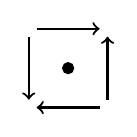
\begin{tikzpicture}
            \draw[black, thick, ->] (0, 0.9) -- (0, 0.1);
            \draw[black, thick, ->] (0.1, 1) -- (0.9, 1);
            \draw[black, thick, ->] (1, 0.1) -- (1, 0.9);
            \draw[black, thick, ->] (0.9, 0) -- (0.1, 0);
            \filldraw [black] (0.5, 0.5) circle (2pt);
        \end{tikzpicture}
    \end{figure}
    In this figure, moving from left to right or top to bottom results in a positive partial derivative.
    These partial derivatives are equal, and by our formula the curl will be zero.
    The figure shows this to be correct, as the flow along this point will push it towards the corners, not in a whirlpool, thus we want this situation to be given zero curl, which is consistent with our formula.

    Furthermore, if we take a point with positive curl, and flip all of the vectors around, then our value of curl will be negative.
    This means that the left side moves faster than the right, and the top faster than the bottom, and thus we get clockwise rotation, which is precisely what we want to describe with a negative value of curl,
    so our definition seems like it covers all 3 cases.

    \subsection*{Understanding Green's Theorem}
    Finally, this picture of curl has a surprising result of making Green's theorem very clear.
    Looking at curl as this arrangement of vectors can lend some powerful insight as to why the theorem is true.
    Observe the following figure.

    \begin{figure}[!h]
        \centering
        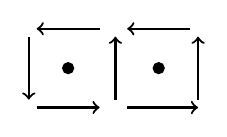
\begin{tikzpicture}
            \draw[black, thick, ->] (0, 0.9) -- (0, 0.1);
            \draw[black, thick, ->] (0.9, 1) -- (0.1, 1);
            \draw[black, thick, ->] (1.1, 0.1) -- (1.1, 0.9);
            \draw[black, thick, ->] (0.1, 0) -- (0.9, 0);
            \filldraw [black] (0.5, 0.5) circle (2pt);
        
        
            % \draw[black, thick, ->] (1.15, 0.9) -- (1.15, 0.1);
            \draw[black, thick, ->] (2.05, 1) -- (1.25, 1);
            \draw[black, thick, ->] (2.15, 0.1) -- (2.15, 0.9);
            \draw[black, thick, ->] (1.25, 0) -- (2.15, 0);
            \filldraw [black] (1.65, 0.5) circle (2pt);
        \end{tikzpicture}
    \end{figure}
    Imagine that this figure represents a very small domain of two points.
    The curl of these two points is very positive, as they both have (roughly) the whirlpool arrangement of vectors we observed earlier.

    However, look at the inner vector.
    In computing the curl, the left point expects that to point up, which it does,
    but the right point expects it to point down, which it doesn't.
    \begin{figure}[!h]
        \centering
        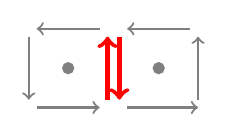
\begin{tikzpicture}
            \draw[gray, thick, ->] (0, 0.9) -- (0, 0.1);
            \draw[gray, thick, ->] (0.9, 1) -- (0.1, 1);
            \draw[red, ultra thick, ->] (1, 0.1) -- (1, 0.9);
            \draw[gray, thick, ->] (0.1, 0) -- (0.9, 0);
            \filldraw [gray] (0.5, 0.5) circle (2pt);
        
        
            \draw[red, ultra thick, ->] (1.15, 0.9) -- (1.15, 0.1);
            \draw[gray, thick, ->] (2.05, 1) -- (1.25, 1);
            \draw[gray, thick, ->] (2.15, 0.1) -- (2.15, 0.9);
            \draw[gray, thick, ->] (1.25, 0) -- (2.15, 0);
            \filldraw [gray] (1.65, 0.5) circle (2pt);
        \end{tikzpicture}
    \end{figure}
    The vectors highlighted in red show how the computation of curl at each point is expecting those vectors, and they oppose.
    When you add the curl of those two points up, you can imagine that expectation canceling those two vectors out.
    And if you cancel those vectors out, you are left with the following figure.
    \begin{figure}[!h]
        \centering
        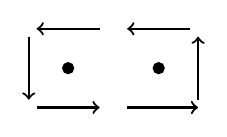
\begin{tikzpicture}
            \draw[black, thick, ->] (0, 0.9) -- (0, 0.1);
            \draw[black, thick, ->] (0.9, 1) -- (0.1, 1);
            \draw[black, thick, ->] (0.1, 0) -- (0.9, 0);
            \filldraw [black] (0.5, 0.5) circle (2pt);
        
            \draw[black, thick, ->] (2.05, 1) -- (1.25, 1);
            \draw[black, thick, ->] (2.15, 0.1) -- (2.15, 0.9);
            \draw[black, thick, ->] (1.25, 0) -- (2.15, 0);
            \filldraw [black] (1.65, 0.5) circle (2pt);
        \end{tikzpicture}
    \end{figure}
    Note that all that is left are the outside vectors, which make up the boundary of the domain.
    Now imagine that you tile many of these squares together all at once.
    All of the internal vectors will cancel, and you will be left with only the exterior vectors.
    If you were to take a line integral over the boundary of that domain it would hit all of those exterior vectors, which are exactly the vectors we are left with after adding up the curl of all of the points.
    We can see that line integral is equivalent to adding up the curl of each point inside the domain,
    as only the outer vectors remain after adding up all of the internal curls.
    The line integral will calculate a curl of its own, of sorts, as it calculates how the flow is 'curling' around the curve, and the double integral of curl over the domain is making the same computation by adding up all of the curls of every point, and canceling the ones that aren't on the boundary.
    This is exactly the statement of Green's theorem, that the double integral of curl over a domain is the same as the line integral of the boundary of that domain.

    This intuition is helpful for understanding what happens when the domains are not simply connected as well.
    It becomes clear that if you remove a segment of your domain, some of those internal vectors that are canceled by adding up every point in the domain should not be canceled if they border the region that has been removed from the domain.
    It is clear then that you simply subtract from your outer line integral the line integral of the boundary of the inner region, as the removed region represents some domain itself that can have Green's theorem applied to it.

    \subsection*{Approximating Partial Derivatives With a Computer}
    In the vector field animation, you are able to click any point to see its calculated divergence and curl.
    To compute these quantities, we need partial derivatives of a vector field.
    A human would symbolically compute the partial derivatives of the vector field, and plug in numbers accordingly, but this animation does not run on symbolic computations.
    Instead it approximates a derivative.

    The process is rather simple, a partial derivative is the change in a quantity as you vary one of its variables.
    When we compute curl, we are interested in $\frac{\partial Q}{\partial x}$ and $\frac{\partial P}{\partial y}$.
    $P$ and $Q$ represent the $x$ and $y$ components of vectors in the field, respectively.
    Knowing this, we can approximate a derivative by taking a point $P_o$, picking a point to the left and a point to the right of $P_o$, and computing the vector field at both of those points.
    We subtract the second y component from the first, and divide by the distance of the two points, and we can successfully approximate $\frac{\partial Q}{\partial x}$, and we can use a similar approach to find $\frac{\partial P}{\partial y}$.

    In notation we may write this as
    \begin{gather*}
        \frac{\partial Q}{\partial x} = \lim_{\Delta x \to 0} \frac{\vec{\mathbf{F}}(P_o + (\Delta x, 0)) - \vec{\mathbf{F}} (P_o - (\Delta x, 0))}{2\Delta x} \boldsymbol{\cdot} \hat{j}
    \end{gather*}
    I had largely forgotten this limit definition until it was necessary to use in a computer based computation.

    Using this, you can arrive at a reasonable approximation for curl, and I will next show how close the approximation is to a real value.
    If we click the point with high curl near the middle, it lies at $(-1, 1.5)$.
    The computer approximates the curl at this point to be roughly $3$, let's see how correct it is.
    \begin{figure}[h]
        \centering
        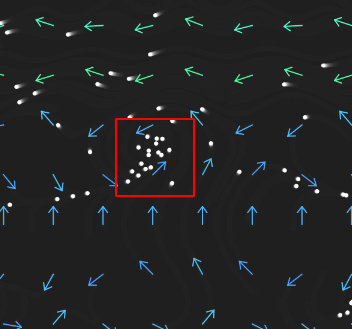
\includegraphics[width=0.5\textwidth]{2020-11-19_12-25}

        This point, $(-1, 1.5)$, is the one in question. It is difficult to see in a still picture, but particles rotate counterclockwise in this region.
        This can be roughly seen from the vectors surrounding it
    \end{figure}

    Our vector field is given by $\vec{ \mathbf{F} } (x, y) = (y \cos(y), \cos(xy))$, and to compute curl we take $\frac{\partial Q}{\partial x} - \frac{\partial P}{\partial y}$. 
    \begin{align*}
        \frac{\partial Q}{\partial x} &= -y\sin(xy) \\ 
        \frac{\partial P}{\partial y} &= \cos(y) - y\sin(y)
    \end{align*}

    To compute curl we subtract these, so our expression for curl is 
    \begin{gather*}
        -y\sin(xy) - \cos(y) + y\sin(y)
    \end{gather*}

    We evaluate this at the point $(-1, 1.5)$, thus our curl is equal to 
    \begin{gather*}
        -1.5\sin(-1.5) - \cos(1.5) + 1.5\sin(1.5) 
    \end{gather*}
    Which comes out to $2.921748$, quite close to the computer's approximation of $3$.

    \section{Conclusion}
    We have seen herein two animations with some surprising insights.
    The first was an animation of parametric coordinates that helped us think of the concept of the 'velocity' of a graph being drawn,
    and how thinking of polar curves having a 'velocity' to them can help us understand when they might draw over themselves multiple times.

    Secondly, we saw an animation of a vector field, that upon observation showed that when a point has high curl, the vectors around that point look like a whirlpool.
    Having observed this, we could derive the formula for two dimensional curl, and use that same picture to understand Green's theorem by canceling the internal vectors
    when you tile many 'whirlpool' points together.

    Combining these, the power of physical or geometric intuition is understood, as many mathematical concepts revealed themselves to be
    very clear when you have the right picture to view.
    While none of these intuitions are proofs of Green's theorem or the definition of curl,
    they do help a user of math better understand the ideas behind what motivates it,
    which can be immediately useful for remembering and extending beyond just what is written in a textbook.

    \section{Works Used}
    The section on Understanding Green's Theorem was heavily inspired by \href{https://www.khanacademy.org/math/multivariable-calculus/greens-theorem-and-stokes-theorem/greens-theorem-articles/a/greens-theorem}{this KhanAcademy article}
    on Green's theorem, which is where I first read about the whirlpool arrangement of vectors.
\end{document}